%%%%%%%%%%%%%%%%%%%%%%%%%%%%%%%%%%%%%%%%%%%%%%%%%%%%%%%%%%%%%%%%
%%%%%%%%%%%%%%%%%%%%%%%%%%%%%%%%%%%%%%%%%%%%%%%%%%%%%%%%%%%%%%%%
%%%%
%%%% This text file is part of the source of 
%%%% `Introduction to High-Performance Scientific Computing'
%%%% by Victor Eijkhout, copyright 2012
%%%%
%%%% This book is distributed under a Creative Commons Attribution 3.0
%%%% Unported (CC BY 3.0) license and made possible by funding from
%%%% The Saylor Foundation \url{http://www.saylor.org}.
%%%%
%%%%
%%%%%%%%%%%%%%%%%%%%%%%%%%%%%%%%%%%%%%%%%%%%%%%%%%%%%%%%%%%%%%%%
%%%%%%%%%%%%%%%%%%%%%%%%%%%%%%%%%%%%%%%%%%%%%%%%%%%%%%%%%%%%%%%%

Another important topic in high performance computers is their power
consumption. Here
we need to distinguish between the power consumption of a single
processor chip, and that of a complete cluster.

As the number of components on a chip grows, its power consumption
would also grow. Fortunately, in a counter acting trend,
miniaturization of the chip features has simultaneously been reducing
the necessary power. Suppose that the feature size~$\lambda$ (think:
thickness of wires) is scaled down to $s\lambda$ with~$s<1$. In order
to keep the electric field in the transistor constant, the length and
width of the channel, the oxide thickness, substrate concentration
density and the operating voltage are all scaled by the same factor.

This is known as \emph{constant field scaling}\index{field scaling} or
\indexterm{Dennard scaling}~\cite{Bohr:30yearDennard,Dennard:scaling},
and it can be considered the driving force behing \indexterm{Moore's
  law}, which states that the number of transistors in a processor
doubles every 18 months.

The net result
is that the dynamic power consumption $P$ is scaled to~$s^2P$ ,
circuit delay $T$ is scaled to~$sT$, and operating frequency $F$ is
changed to~$F/s$.Correspondingly, the energy consumption is scaled
by~$s^3$, and this gives us the space to put more components on a
chip.

At the time of this writing (circa~2010), miniaturization of
components has almost come to a standstill, because further lowering
of the voltage would give prohibitive leakage. Conversely, the
frequency can not be scaled up since this would raise the heat
production of the chip too far. 
%
\begin{figure}[ht]
  \begin{quote}
  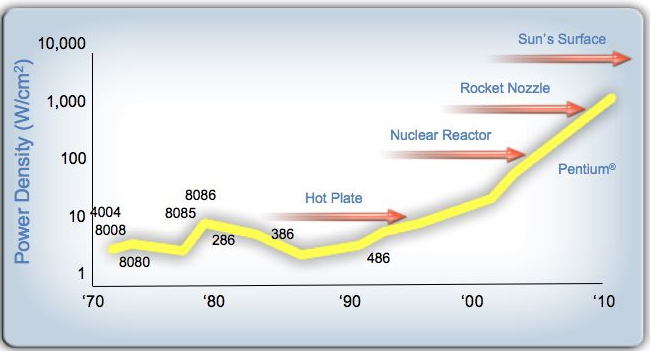
\includegraphics[scale=.6]{graphics-public/chipheat0}
  \end{quote}
  \caption{Projected heat dissipation of a CPU if trends had
    continued -- this graph courtesy Pat Helsinger}
  \label{fig:chipheat}
\end{figure}
%
Figure~\ref{fig:chipheat} gives a dramatic illustration of the heat
that a chip would give off, if single-processor trends had
continued.

One conclusion is that computer design
is running into a \indextermbus{power}{wall}, where the sophistication
of a single core can not be increased any further (so we can for
instance no longer increase \indexac{ILP} and
\indextermbus{pipeline}{depth}) and the only way to increase
pwerformance is to increase the amount of explicitly visible
parallelism. This development has led to the current generation of
\indexterm{multicore} processors; see section~\ref{sec:multicore}. It
is also the reason \acp{GPU} with their simplified processor design
and hence lower energy consumption
are attractive; the same holds for \acp{FPGA}.

We can characterize this shift as one from larger cores, higher
frequency, and higher power, to one where process technology, larger
integration, and new micro-architectures come together for more
power-efficient performance~\cite{Bohr:ISSCC2009}.

The total power consumption of a parallel computer is determined by
the consumption per processor and the number of processors in the full
machine. At present, this is commonly several Megawatts. By the above
reasoning, the increase in power needed from increasing the number of
processors can no longer be offset by more power-effective processors,
so power is becoming the overriding consideration as parallel
computers move from the petascale (attained in 2008 by the
\indextermbus{IBM}{Roadrunner}) to a projected exascale.

In the most recent generations of processors, power is becoming an
overriding consideration, with influence in unlikely places. For
instance, the \ac{SIMD} design of processors (see
section~\ref{sec:simd}, in particular section~\ref{sec:sse-avx}) is
dictated by the power cost of instruction decoding.
